%for reference to this section
\section{Introduction}
\label{section:Introduction}
Eye tracking has been a valuable research method for over one hundred years \autocite{biedert2010eyebook}. Popular search engines like Google and Yahoo! also profit from that sort of research. When a user enters a query and afterward looks at the corresponding search engine result page (SERP), they mostly only pay attention to the first few results and probably do not look at the second recommended result page \autocite{lorigo2008eye, liu2015influence}.\\
Therefore, the goal of this paper is to understand the user's viewing and reading behavior better. As a consequence, the user experience can be improved by adjusting the interface of the search engine result page. This will also allow the user to execute more efficient research tasks with the help of a search engine.\\
This paper will look further into eye tracking to achieve the goal of improving SERPs. In particular, the essential eye tracking technologies, parameters and visualization methods to optimally illustrate the gathered results. Moreover, this paper will describe what a commonly used search engine nowadays looks like and how it can be improved.


\section{Reading}
\label{section:Reading}
There has been done a lot of research, particularly in the field of psychology, in the last century about information processing, first and foremost reading \autocite{rayner1998eye, biedert2010eyebook}. 
To better understand the reader and adjust any kind of reading material or just a simple text as accurate as possible to the reader, it is essential to understand the user's reading behavior \autocite{biedert2010eyebook}. 
Therefore, this following section will include the most relevant information regarding the human's eye and its movements, information processing -- in particular reading -- and individual differences or challenges that may appear when it comes to reading.

\subsection{Eye}
\label{subsection:Eye}
As the eye is responsible for starting the mechanism of processing all kinds of visual stimuli coming from our environment, it is necessary to understand how the human eyes are structured and how they function. Accordingly, this following section will cover the eyes physiological architecture and the movements that the eyes perpetually execute.

\begin{figure}[!ht]
    \centering
    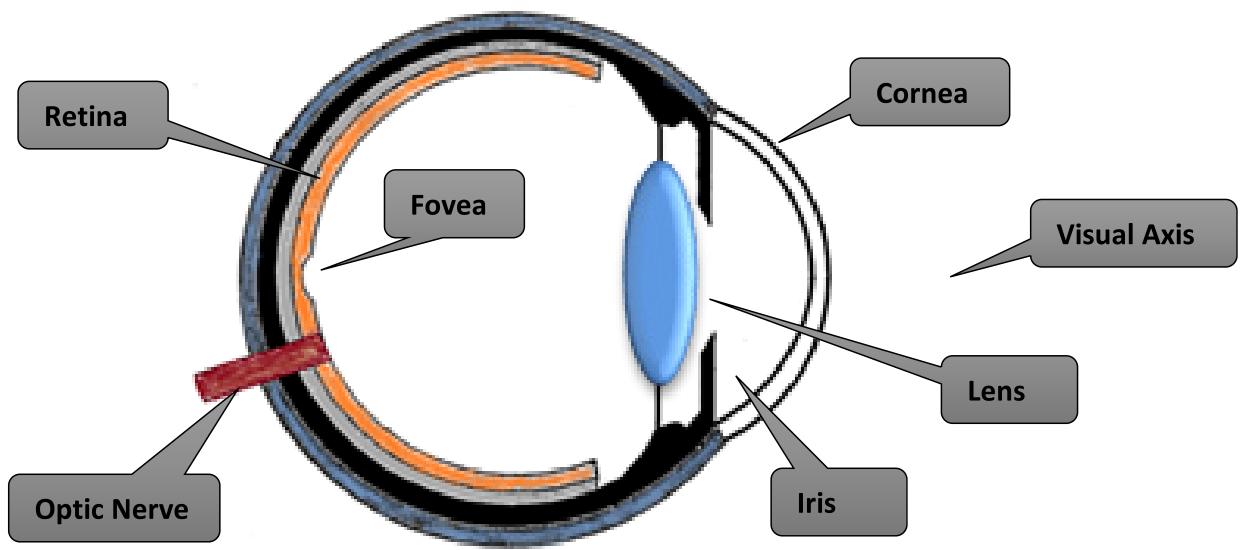
\includegraphics[width=0.75\linewidth]{images/Eye_djamasbi2014eye.png}
    \caption{
       Structure of the eye \autocite[38]{djamasbi2014eye}
    }
    %for reference to this figure
    \label{figure:Eye}
\end{figure}

\subsubsection{Physiological}
A human eye (see Figure \ref{figure:Eye}) consists of various parts such as the cornea, the lens, the iris, the fovea and the retina \autocite{djamasbi2014eye}. When a human looks at an object, the first thing that happens is that the light reflects off the object and hits the front region of the eye, also known as the cornea. After that, the reflected light travels through the iris and lens and hits the back of the eye, which is called the retina. Inside of the retina are the two visual receptors, called the rods and the cones. These receptors are not evenly distributed. There are fewer cones, that deliver the best results in bright and illuminated environments, as they are especially and entirely responsible for distinguishing colors, acuity and identifying detail. Which means there exists a larger number of rods since their main purpose is to differentiate between grey shades and brightness levels and also identify movements. In contrast to the cones, rods function at its best when the environment is only slightly illumined \autocite{djamasbi2014eye, biedert2010eyebook}.
When a beam of light hits the retina, it most likely arrives at the foveal area, which is the part of the retina where most of the cones are located at \autocite{djamasbi2014eye}. Consequently, the fovea is also partly responsible for a precise vision \autocite{biedert2010eyebook}.
Moreover, when the reflected light reaches the back of the eye, the receptors convert the light signal into an electrical and also neural signal. Through the nerves, this signal gets sent to the brain where it can be further processed \autocite{djamasbi2014eye}.

\subsubsection{Movements}
As \textcite{djamasbi2014eye} is explaining in their paper the best acuity, concerning seeing, occurs with the help of the fovea -- contains the highest number of cones. Outside of that area, the visual acuity decreases immensely. To compensate these disadvantages, the human eye automatically executes a lot of quick ballistic movements between two points. These fast movements are called saccades and regressions.
Aside from that, when the eyes are not moving at such fast pace, they mostly fixate on certain words, objects or areas. However, \textcite{biedert2010eyebook} mention in their paper that when the eye is fixated at a point, it can only ingest a limited amount of information.

In addition, \textcite{bruneau2002eyes} mentions that most eye movements seem to happen not voluntary. Therefore, recording the eyes with a tracking device can collect unbiased information about how the human observes and interacts with any sort of system. In contrast to that, \textcite{clifton2016eye} suggest that eye movements have a close relation to lexical and other linguistic processing and maybe even are completely controlled.

\subsection{Information Processing}
\label{subsection:InformationProcessing}

As \textcite{laberge1974toward} were already explaining in their paper, the skill of reading can be divided into different stages of information processing. There are also several stages when it comes to improving the reading skills over time, e.g., become a better and ideally fluent reader. Nevertheless, the critical part is the action that happens during the reading process. For a fluent reader, the information processing happens within small fractions of a second. For beginners, the processing can last longer than that, but this skill can be trained and thus can also be improved \autocite{laberge1974toward}.

As \textcite{biedert2010eyebook} explain in their study, cognitive processes of the brain, for example information processing, and eye movements are closely related.  As a consequence, when the human's eye movements are being recorded and the movements are interpreted, personal reading behavior can be extracted and further estimated \autocite{biedert2010eyebook}.

Moreover, \textcite{buscher2009you} discovered in their study that there is more information processed if a specific point is looked at more prolonged than the average amount of time. Regardless, the brain can only process a finite amount of information at the same time \autocite{biedert2010eyebook}.

\subsection{Individual Differences and Challenges}
\label{subsection:Differences}
\textcite{rayner1998eye} lists a handful of individual differences that distinguish readers from one another. For example, fast and slower readers, bilingualism, stuttering and dyslexia. Experienced readers do not have to reread sections as often and get faster through a text. Bilingual people also have different reading patterns depending on the language the text is written in, e.g., they read texts faster if they are written in their mother tongue. Furthermore, people who stutter have a harder time reading a text than non-stuttering people \autocite{rayner1998eye}. 
In addition, dyslexic people tend to generally need more time to read a text, which does not automatically mean that they make more mistakes than normal readers while reading \autocite{rayner1998eye, hutzler2004eye}.
In their study \textcite{hutzler2004eye} found that their participants had more difficulties with larger words than the average reader.
Moreover, they found out that there are differences in various languages similar to bilingual readers \autocite{hutzler2004eye, rayner1998eye}.

\section{Eye Tracking}
\label{section:EyeTracking}
When an eye tracking device is being used, someone's eye movements are being recorded. This recorded material, the raw eye tracking data, can be evaluated and the resulting parameters (e.g., fixation, saccades, regression, etc.) can be summed up in visualization graphs \autocite[]{goldberg2002eye, poole2006eye, beymer2007eye}. Hence, eye tracking can be used as a valuable tool in many web application cases such as creating webpages, placing advertisements or arranging search engine result pages \autocite{buscher2009you, liu2015influence}. \textcite[]{buscher2009you} note in their paper that web developers can also profit from taking eye tracking study results into consideration when designing and styling their new websites. 

However, eye tracking is not only used for webpages. For instance, another outstanding application case is psychology, where the eye tracker is used to record the eye movements while doing any kind of information process, e.g. reading \autocite{schiessl2003eye}.
Accordingly, when it comes to online reading, eye tracking has been a helpful expedient to gain information on how the human brain processes information retrieved from a text \autocite[]{schiessl2003eye}.
As a result, the following section will include the most popular technologies, parameters and accordingly the required visualization methods. 

\subsection{Technologies}
\label{subsection:Technologies}
As \textcite[]{biedert2010eyebook} is expressing in their paper, eye tracking has been around for more than 100 years, and researchers gained a lot of important data. As a consequence, eye tracking technology has evolved a lot over these several years \autocite[]{poole2006eye}.
For example, in the time since the first eye tracking devices have been invented, they have come a long way. In the early beginnings, direct contact with the cornea was necessary as \textcite[]{jacob2003eye} mention in their paper.
Accordingly, this next section will cover several essential facts and changes when it comes to eye tracking technology.

\subsubsection{Head-mounted vs. remote}
To record a subject's eye movements, there are two kinds of eye tracking devices available. The first one is called head-mounted. This kind of apparatus is placed on the subject's head and therefore always requires contact as seen in Figure \ref{figure:HeadMounted}. 
The second one, also called a remote device, does not require contact and for that reason, it is most commonly placed next to or on top of the computer screen where the desired content is being displayed \autocite[]{jacob2003eye, schiessl2003eye}. In this example (see Figure \ref{figure:HeadMounted}), the camera is integrated into the monitor right below the screen as well as the infrared light source. 
To calibrate the camera correctly, a short process is necessary, where the user usually has to fixate points on different locations on the screen for a short period of time \autocite{biedert2010eyebook}.

\begin{figure}[!ht]
    \centering
    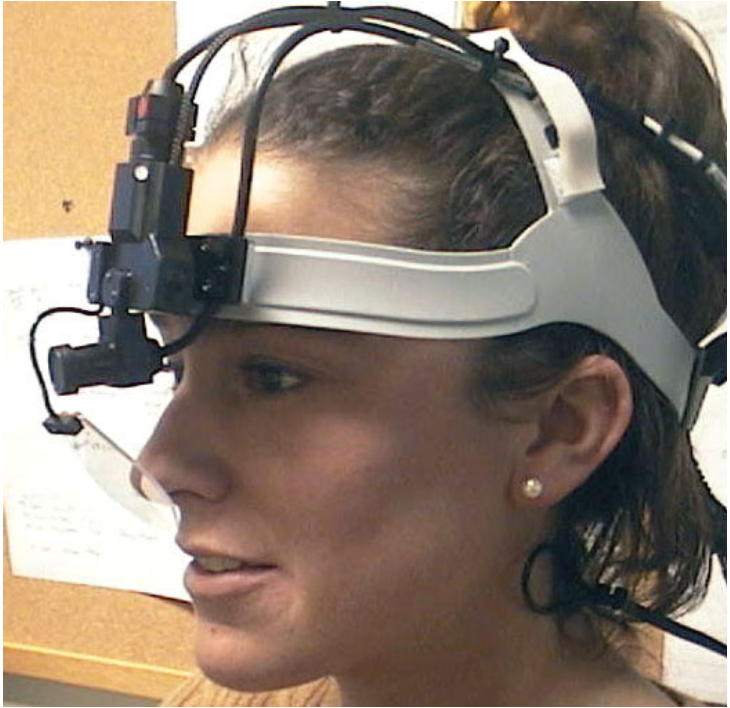
\includegraphics[width=0.75\linewidth]{images/headmounted_goldberg2002eye.png}
    \caption{
        Example of a head-mounted eye tracking device \autocite[12]{goldberg2002eye}
    }
    %for reference to this figure
    \label{figure:HeadMounted}
\end{figure}

\begin{figure}[!ht]
    \centering
    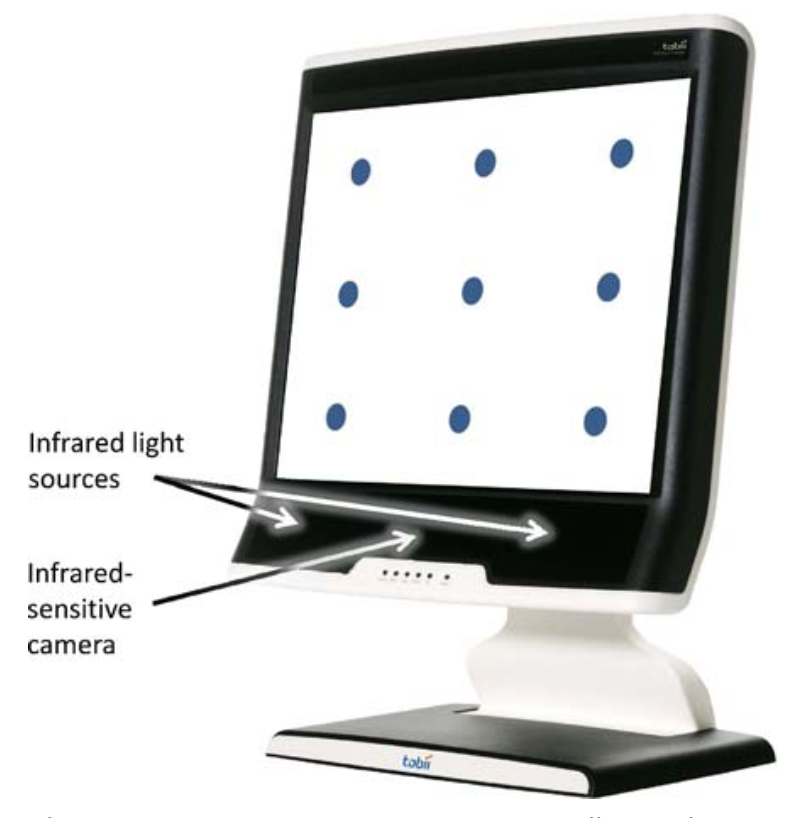
\includegraphics[width=0.75\linewidth]{images/remote_biedert2010eyebook.png}
    \caption{
        Modern example of an remote eye tracker \autocite[274]{biedert2010eyebook}
    }
    %for reference to this figure
    \label{figure:Remote}
\end{figure}

\subsubsection{Infrared light -- bright and dark pupil}
While using a remote eye tracking device to record someone's eye movements, the camera most likely uses infrared light as an illuminator. Thus, the light hits the front of the eye which is also called the cornea and afterward the back, the retina. 
Moreover, the reason why the infrared light is used instead of any other light source is that it would distract the user while viewing the test material \autocite[]{poole2006eye, biedert2010eyebook}.

The two most known techniques, as mentioned by \textcite[]{goldberg2002eye}, are known as the bright and the dark pupil method. The bright pupil has the infrared placed in the same axis and ideally the same place as the camera. Therefore, the pupil is illuminated and brighter than the iris (this exact same effect leads to red eyes photos). The second method, dark pupil, has the illumination source placed on a different axis as the camera recording the eye. That leads to the pupils being darker (see Figure \ref{figure:DarkBright}). To gain improved results, these two methods can be used within the same eye tracking device \autocite[]{tobii2018dark, goldberg2002eye}. 

\begin{figure}[!ht]
    \centering
    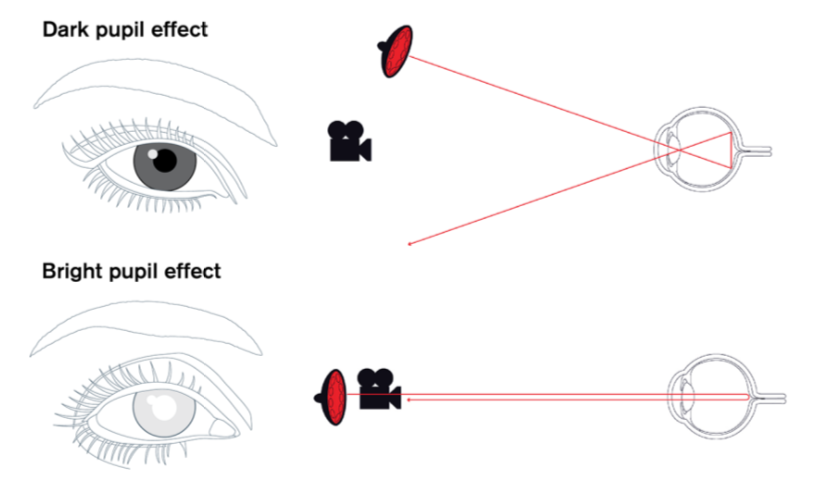
\includegraphics[width=1\linewidth]{images/DarkBright.png}
    \caption{
        Illustration of dark and bright pupil method  \autocite[]{tobii2018dark}
    }
    %for reference to this figure
    \label{figure:DarkBright}
\end{figure}


\subsection{Parameters}
\label{subsection:Parameters}
When an eye tracking device records a subject's eye movements, raw data can be collected. For instance, the most common element can be gaze points, which are points that get visually focused by the human's eye \autocite{bojko2009informative, vspakov2007visualization}. To extract valuable and applicable information out of the obtained raw data, \textcite[]{blascheck2014state}  suggests to aggregate it into fixations and saccades. 
Nowadays those are the two most commonly used parameters \autocite{bruneau2002eyes}. Thus, this section will provide a brief overview of the most essential and relevant parameters.

\subsubsection{Fixations}
A fixation is understood as a steady gaze at one point \autocite[]{buscher2009you}.  In the context of reading, as \textcite[]{beymer2007eye} annotate in their paper, fixations are moments where the gaze is paused on a word or a group of words. 
Normally a fixations duration lasts about 200-300 ms \autocite[]{kasneci2015online}. As stated by \textcite[]{buscher2009you}, to be considered a fixation the gaze must at least last 80-100 ms. Accordingly, during that time the brain can process the ingested information. Aside from that, a field where many foveal fixations take place is called an area of interest (AOI) \autocite[]{djamasbi2014eye}. For example, a webpage can be divided into different areas of interest (see Figure \ref{figure:AOI}).  On the one hand, when specific AOI's are used, one area can be simply a picture or the heading of a webpage. On the other hand, using broad AOI's, the page gets partitioned into larger parts like heading, pictures and text \autocite{djamasbi2014eye}. \\

\begin{figure*}[t]
    \centering
    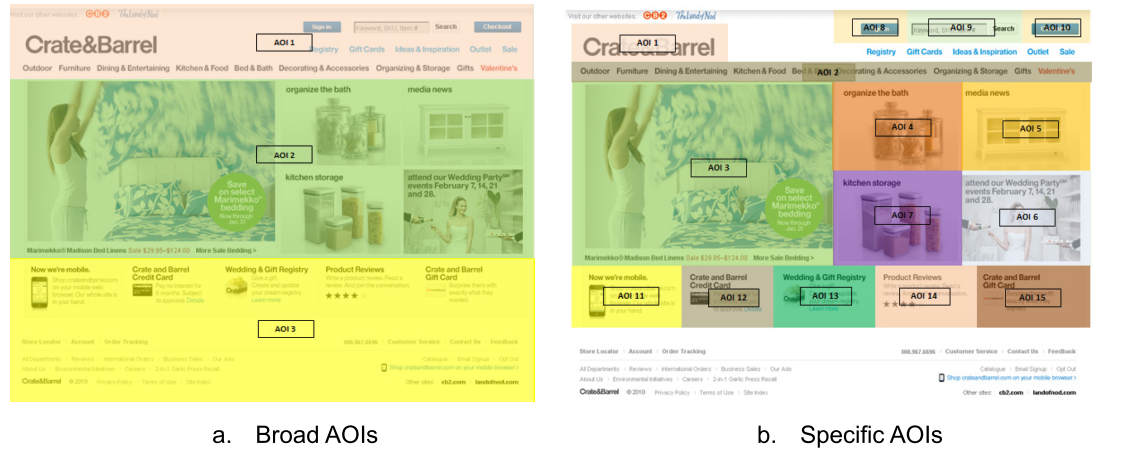
\includegraphics[width=0.75\linewidth]{images/AOI_djamasbi2014eye.png}
    \caption{
        Webpage divided into areas of interest (AOI) \autocite[48]{djamasbi2014eye}
    }
    %for reference to this figure
    \label{figure:AOI}
\end{figure*}

According to \textcite[]{grzyb2016eye}, when a user is looking at a website and an eye tracking device is set up, not all recorded fixations are detected correctly.
For instance \textcite[]{bruneau2002eyes} states in his paper, that not all eye movements seem to happen voluntarily. 
Despite the fact that fixations may not be an entirely flawless eye tracking parameter, \textcite[]{biedert2010eyebook} mention in their paper that information can only be correctly discovered with fixations.

\subsubsection{Saccades and Scanpaths}
Another significant parameter is the saccade which is the counterpart to fixations \autocite{goldberg2002eye}. They are short and fast movements between two points, the before mentioned fixations \autocite{goldberg2002eye, beymer2007eye}. Saccades are the quickest movements the body is able to achieve and typically last 30 to 80 ms \autocite[]{blascheck2014state}. \\
Furthermore, the scanpath is an important metric in terms of fixations and saccades. Scanpaths consist of alternating saccades and fixations. They reveal information about where the user looks first because scanpaths gives information in which order they look at what part of a website. Therefore, it can offer insights into the user's experience and additionally their behavior when they observe or interact with a website \autocite[]{lorigo2008eye, blascheck2014state}. Figure \ref{figure:Scanpath} shows scanpaths on a website, where the dots are the fixations and the lines are the saccades. \\
In the context of reading text on a website, a saccade is habitually a forward movement for around 8-12 characters in the text that is being read as \textcite[]{beymer2007eye} are explaining in their paper.

\begin{figure}[!ht]
    \centering
    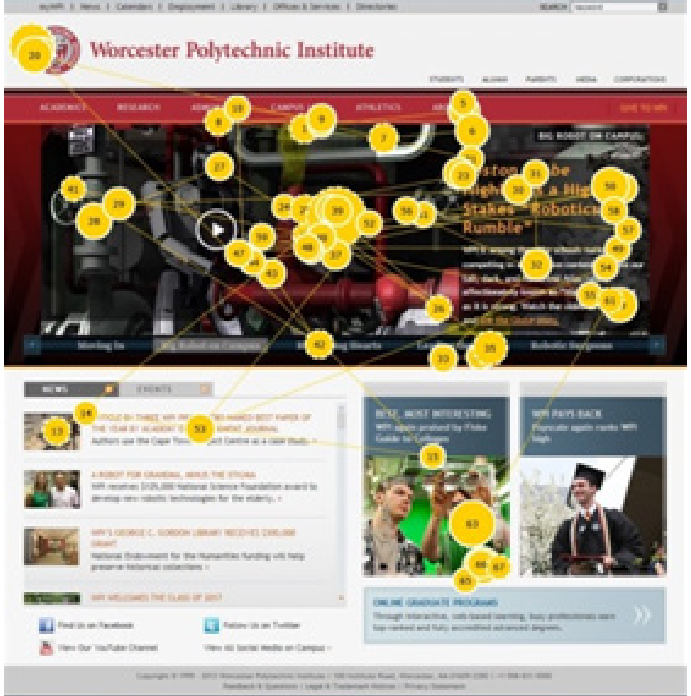
\includegraphics[width=0.75\linewidth]{images/scanpath_djamasbi2014eye.png}
    \caption{
       One possible way to visualize scanpaths \autocite[43]{djamasbi2014eye}
    }
    %for reference to this figure
    \label{figure:Scanpath}
\end{figure}

\subsubsection{Regressions}
Saccades are usually only forward movements, hence fast backward movements are called regressions \autocite[]{reichle1998toward}. 
\textcite[]{rayner1998eye} claims in his paper that regressions add up to 10 - 15 \% of the before mentioned saccades.
While reading a passage of a text, regressions are movements to the left of the line, mostly a few characters back, sometimes earlier words or occasionally even a whole sentence. Therefore \textcite[]{kruger2014subtitles} suggest in their paper that this could be an indicator of having troubles in processing the reading material or merely just oculomotor errors. Although most of the times the reader is not aware of those movements \autocite[]{reichle2003ez, biedert2010eyebook}.

\subsubsection{Pupil size}
As \textcite{goldberg2002eye} is describing in their paper one of the main reasons why someone's pupil size may change is increasing or decreasing illumination. For example, an eye tracking study can include videos or something else that is presented to the subject. If that happens, brightness may change very often in the shown material. As a consequence, the pupil size is constantly altering. To reestablish a more constant pupil size, the brightness of the room can be adjusted \autocite[]{goldberg2002eye}.
For example, the eye's pupil dilation can reveal whether the user finds interest in the website the look at or not. Hence, when the pupil is bigger, the user is also more interested as well as aroused, and when the pupil is smaller, the user does not find much interest in the material \autocite[]{joachims2017accurately}.\\
It is disputed that pupil dilation as a parameter can be an unreliable source because not only the text, but every little detail goes into one's reading experience. For example, sudden sounds in the surrounding area can play a part in one's change of pupil size when reading a text. 
Despite that, pupil dilation in a controlled environment, regarding time and space, can still say a lot about a user's experience on a website \autocite[]{bruneau2002eyes}.

\subsection{Results and Visualization}
\label{subsection:ResultsVisualization}
Once the eye movements of a person got recorded, the raw eye tracking data can be further processed. There are different methods to visualize the various eye tracking parameters. This following section will address today's most commonly used techniques and try to gauge which one is the most efficient.

\subsubsection{Statistical visualization approach}
The first approach for visualizing data are commonly used methods from statistics that are likewise used in eye tracking \autocite{blascheck2014state}. Raw eye tracking is primarily nothing more than mathematical or cartesian coordinates \autocite{blascheck2014state, biedert2010eyebook}. In addition to that, the raw data can contain information about the position of a user's head \autocite[]{biedert2010eyebook}. 
As \textcite[]{blascheck2014state} states in their paper, these statistical approaches are not exclusively constructed for eye tracking data. There are the three following alternatives to visualize the data: line chart, bar chart and scatter plot. The first one is the line chart which mostly displays mini-movements, slides, saccades or the mean time of fixations. The second is a bar chart which is typically used in the form of a histogram where the mean fixation duration is portrayed. And the third and last one is called a scatter plot which often illustrates saccadic movements \autocite[]{blascheck2014state}.
As mentioned before, these three graphs are not explicitly made to visualize eye-tracking data. Therefore they may not be the best option to visualize these specific results.  Although all three graphs (see Figure \ref{figure:Statistics}) represent the same set of data, eye tracking data can be represented in many different ways and may mislead. 

\begin{figure}[!ht]
    \centering
    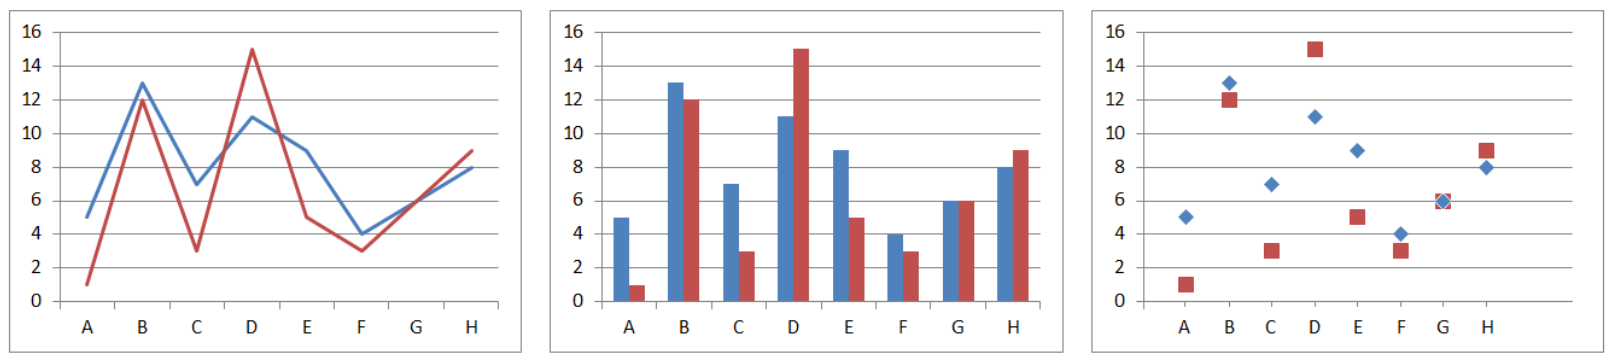
\includegraphics[width=1\linewidth]{images/statistics_blascheck2014state.png}
    \caption{
       Statistical representation of eye tracking data \autocite[7]{blascheck2014state}
    }
    %for reference to this figure
    \label{figure:Statistics}
\end{figure}

\subsubsection{Heat maps}
As the second method, when it comes to visualizing the results of the gathered eye tracking data, one of the most commonly used visualization methods are heat maps. 
\textcite{bojko2009informative} state in their paper that one of the reasons why heat maps are often used is that they are simple to produce. 
A heat map can illustrate the number of fixations by coloring the most looked at points and parts of a website in a two-dimensional graph. Therefore, heat maps receive their name from the colors, which correspond to temperature. For example, red and yellow on the heat map portray the most frequently looked at points (see Figure \ref{figure:HeatMap}) \autocite[]{bojko2009informative}. 

As \textcite[]{bojko2009informative} explains in their paper, heat maps are not a solution for every task that is being recorded with an eye tracking device. 
For example, when heat maps are being used to test if an element is poorly placed on a website. To get more realistic and reliable results, it would be necessary to put the desired item in more than one areas of the website and then repeat the trial. However, this would lead to a comparison between the accumulated data and its heat map, which is also not a reliable source to interpret a user's behavior \autocite[]{bojko2009informative}. 
In addition, according to the study of \textcite[]{djamasbi2010efficiency}, comparing two heat maps is not possible because they are not standardized in the sense of fixation quantity. Although both heat maps illustrate the fixations that were recorded before, the number of the fixations may differ. Therefore, two comparable heat maps must have the same amount of fixations to provide relevant results \autocite[]{djamasbi2010efficiency}. 

Furthermore, heat maps are not always an excellent representation of eye tracking data, because the colors are very opaque so that the original picture on the screen is not clearly visible anymore. To minimize this problem in a lot of studies the heat maps are turned into shadow maps where the image behind the overlapped map is still detectable \autocite[]{vspakov2007visualization}. Another alternative to avoid the opaqueness of heat maps are focus maps (see Figure \ref{figure:FocusMap}) which are similar to shadow maps, where the important and more looked at points are visible and the rest of the picture is black \autocite{kruger2014subtitles}.

\begin{figure}[!ht]
    \centering
    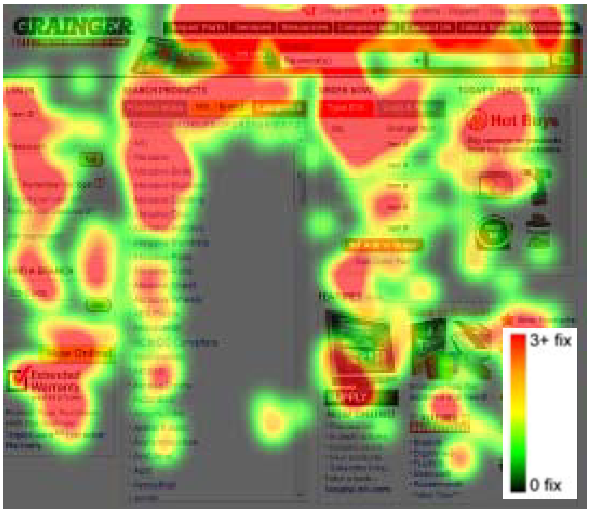
\includegraphics[width=0.75\linewidth]{images/HeatMap_bojko2009informative.png}
    \caption{
       Exemplar of a heat map from a website \autocite[32]{bojko2009informative}
    }
    %for reference to this figure
    \label{figure:HeatMap}
\end{figure}

\begin{figure}[!ht]
    \centering
    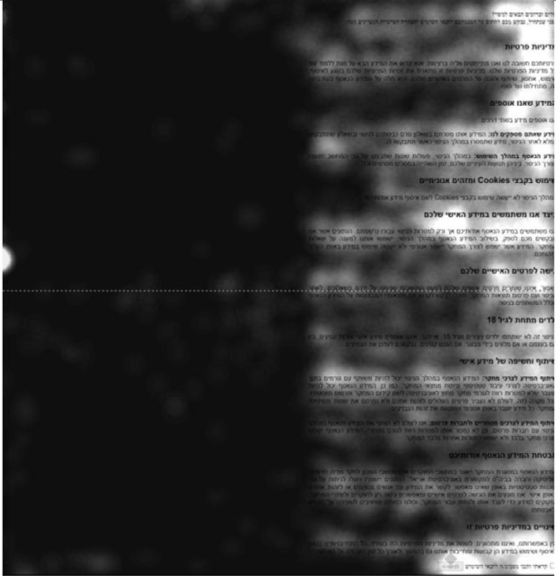
\includegraphics[width=0.75\linewidth]{images/focusMap_steinfeld2016agree.png}
    \caption{
       Focus map of users reading privacy policies online (written in Hebrew, right-to-left) \autocite[997]{steinfeld2016agree}
    }
    %for reference to this figure
    \label{figure:FocusMap}
\end{figure}

\subsubsection{Area of interest map}
An area of interest, in the context of websites, is a part of a webpage where plenty of fixations are recorded. To visualize and group them in the best way possible, a website can be divided into regions or areas of interest. These regions are either specific (e.g., items like buttons, pictures, advertisements) or rather global (e.g., top, middle, bottom of a webpage) and wide (see Figure \ref{figure:AOI}) \autocite[]{gonzalez2011different, djamasbi2014eye}. To gain more information about a website and how a user views it a fixation duration map and the areas of interest map are combined.
\textcite{djamasbi2014eye} is observing in their paper, that this resulting map can provide a lot of information, for example, whether or not a specific part of a website is exciting for the user or if users pay attention to it in general or if a part of the website may get overlooked a lot. Furthermore, with the help of fixation timing, an AOI map can give information about the order in which the user views a webpage \autocite[]{djamasbi2014eye}.
An example of dividing a webpage into AOI's can be seen in Figure \ref{figure:AOI}b. The page is partitioned into specific areas like the heading, the menu bar, the main picture, other pictures with small headings and abstracts, the sign-in area and the search bar. When a fixation map and an AOI map are combined, the result reveals information about the fixation duration the user assembled \autocite{djamasbi2014eye}.

\subsubsection{Gaze plot}
A third approach to visualizing eye-tracking data is using gaze plots. Similar to the already mentioned attention maps, to be exact heat maps, gaze plots also use information about a user's fixation \autocite[]{kurzhals2016gaze}. \textcite[]{kurzhals2016gaze} also mentions that gaze points not only display fixations but also take scanpaths, alternating fixations and saccades, into account. 

\begin{figure}[!ht]
    \centering
    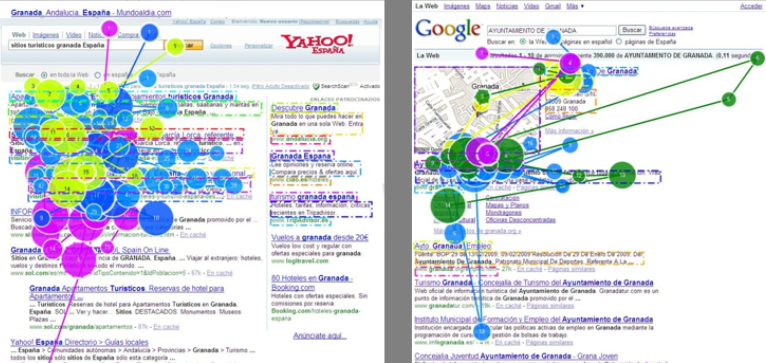
\includegraphics[width=1\linewidth]{images/GazePlot_gonzalez2011different.png}
    \caption{
       Another example of gaze plots arranged for the same type of query \autocite[12]{gonzalez2011different}
    }
    %for reference to this figure
    \label{figure:GazePlot}
\end{figure}

As seen in Figure \ref{figure:GazePlot}, gaze plots are an ideal visualization method for scanpaths, therefore also for fixations and saccades. In a gaze plot, the points represent the fixations. The larger the point the longer that position was fixated by the user. The lines between those fixations points serve as a representation of the saccadic movements of the human's eyes \autocite[]{djamasbi2014eye}.
As a consequence, similar to heat maps, gaze plots have dots all over the place, and the whole view is clustered with them. Therefore, the picture with all its items behind is often not clearly visible anymore as \textcite[]{djamasbi2014eye} indicates in their paper.

\subsubsection{Gaze stripes}
And lastly, there is another method that is called gaze stripes and is image-based. There are two input forms necessary for creating gaze stripes as \textcite{kurzhals2016gaze} is explaining in their paper. Firstly, there is the visual attention that gets examined by the user. And secondly, gaze stripes consist of the spatio-temporal information about coordinates the eye tracking device records \autocite{kurzhals2016gaze}.

\textcite[]{kurzhals2016gaze} introduce a new kind of visualization method (see Figure \ref{figure:GazeStripes}. This method does not require pre-defined areas of interest because it uses the image around the gaze point. The method will work for static as well as dynamic sensory input. 

Furthermore, it will make it more accessible to interpret scanpaths. However, this method brings one issue along. For example, if the used stimuli contain similar colors, it becomes hard to differentiate between the separate objects in the picture \autocite[]{kurzhals2016gaze}.

\begin{figure}[!ht]
    \centering
    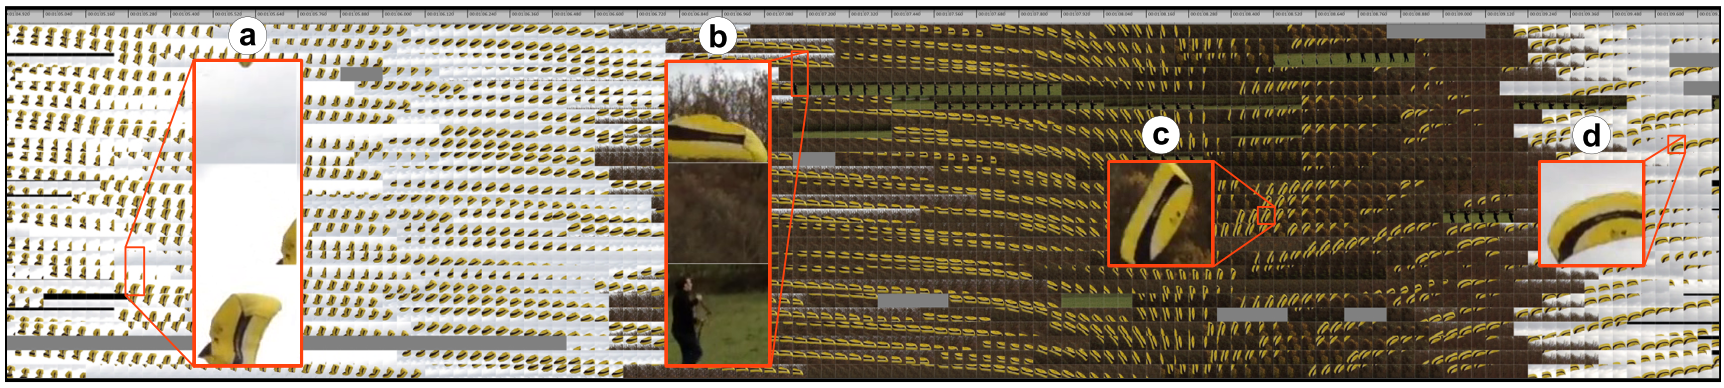
\includegraphics[width=1\linewidth]{images/GazeStripes_kurzhals2016gaze.png}
    \caption{
       Another example of heat maps and gaze plots  arranged for the same queries \autocite[1005]{kurzhals2016gaze}
    }
    %for reference to this figure
    \label{figure:GazeStripes}
\end{figure}


%SEARCH ENGINE - SEARCH ENGINE - SEARCH ENGINE - SEARCH ENGINE - SEARCH ENGINE - SEARCH ENGINE
\section{Application Case -- Search Engine (Search Engine Result Pages)}
\label{section:SearchEngine}
This following chapter will discuss the previously collected knowledge concerning information processing and eye tracking. Furthermore, search engines and the associated search engine result pages will be taken into account as one of many possible application cases when it comes using eye tracking as a research method.

\subsection{Information Processing and SERP}
\label{subsection:ReadingSERP}
When it comes to search engines, there has been done a lot of research to optimize the presentation of the results that are shown on the result page.  In order to enhance the user's experience, e.g., display the most appropriate and relevant links at the top, and adjust the SERP as good as possible, it is essential to understand how the user observes the result page \autocite{buscher2010good, liu2015influence}.
For the longest time, displaying only websites as the results is a search engine's most important purpose. Besides, a search engine also presents advertisements, maps, images, videos, news and more results on their search engine result page. Nowadays, when mainly considering the links to webpages and their corresponding abstracts, which is the first page a user sees after entering a query and also the main result page of the search engine, a SERP is essentially built the same way as seen in Figure \ref{figure:ModernSerp}.
The result page contains elements like the search bar and button, advertisements with links and abstracts, fundamental links to webpages that match the search query, pictures and links to videos \autocite{wang2016beyond}.

\begin{figure}[!ht]
    \centering
    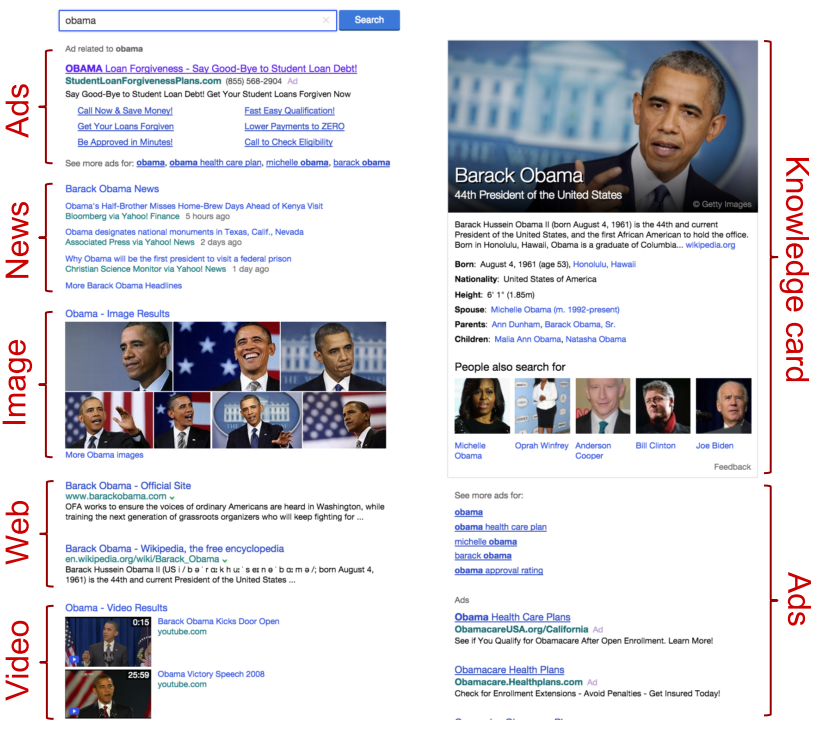
\includegraphics[width=1\linewidth]{images/SERP_wang2016beyond.png}
    \caption{
        Example of a modern Search Engine Result Page \autocite[104]{wang2016beyond}.
    }
    %for reference to this figure
    \label{figure:ModernSerp}
\end{figure}

As \textcite{lewandowski2015evaluating} is explaining in their paper, a few years ago SERPs were structured differently. For instance, the search engine result pages were built after the "ten blue links"-principle. Hence, those pages generally just consisted of the essential ten links to webpages. Moreover, this principle indicates and reinforces the user's behavior to only look at the first few results that a search engine computes \autocite{lewandowski2015evaluating, liu2015influence, wang2016beyond}. Another way to describe this convention is called "organic results". Accordingly, there is a section with the "organic results" on a SERP with no advertisements featured (see Figure \ref{figure:OrganicResults}) where solely the results and their abstracts get displayed \autocite{buscher2010good}.

\begin{figure}[!ht]
    \centering
    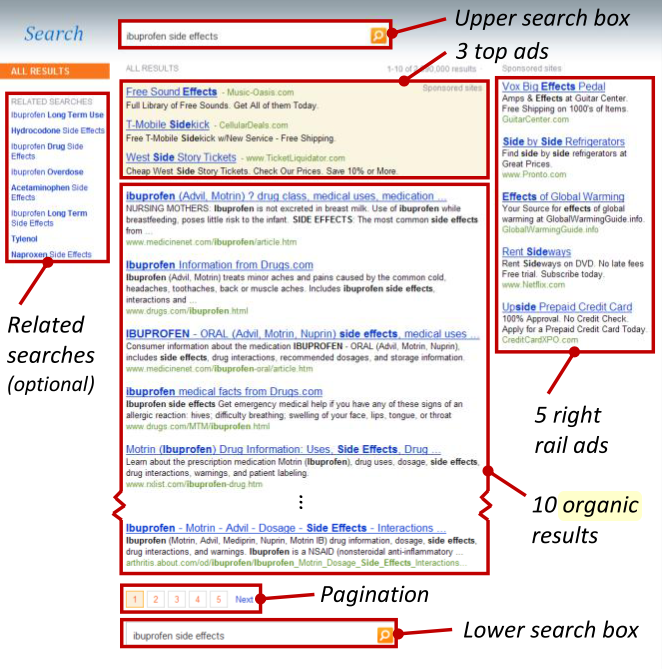
\includegraphics[width=1 \linewidth]{images/organic_buscher2010good.png}
    \caption{
        Example of the "ten blue links" or "organic results" on a modern SERP \autocite[3]{buscher2010good}
    }
    %for reference to this figure
    \label{figure:OrganicResults}
\end{figure}

On a result page that is built after the "ten blue links"-principle the result-links are ranked based on relevance. Therefore, the search engine makes estimations and evaluations itself, whether the user would find the shown results rather fitting or not. This process is also called the "probability ranking principle" \autocite{wang2016beyond}. This policy is reasonably justified because the user usually never reads further than the first suggested page out of the various recommended pages as \textcite{lewandowski2015evaluating} is explaining in their paper.\\
One of the most prominent parts of the website is the section that includes pictures. Furthermore, the human eyes tend to pay increased attention to images in comparison to plain text. When an eye tracking device is being used to record the user's movements,  images get looked at more. This phenomenon is called the attention bias, more specifically the vertical bias \autocite{wang2016beyond}.
The same exact issue seems to appear with the before mentioned "ten blue links" that are summed up into a vertical result \autocite{wang2016beyond}.\\
In contrast, \textcite{liu2015influence} explain in their paper that not all pictures get the same amount of attention. In their study, they found that images that happen to be a part of a preview of news content get overlooked most of the times. Only images that are not directly attached to any sort of article or link get more attention \autocite{liu2015influence}.

To get additional information from the recorded material of the eye tracking device, the raw eye tracking data is evaluated and interpreted. One of the most noticeable and relevant parameters, in the context of information processing and reading, are fixations. They reveal the most relevant information about the human's reading behavior \autocite{pan2007google}. As \textcite{rayner1998eye} is explaining in their paper, only during fixations the brain is able to process information from our environment. Consequently, during saccadic movements, the information intake decreases correspondingly. During these saccades, the eyes move too quickly to receive new data \autocite{rayner1998eye}. 
Therefore, the number of fixations discloses information about how the user processes the read information. In cases of a text that is more difficult, it is assumed that a higher number of fixations correlates to more information being processed. Besides, as mentioned before, pupil size can also be an indicator of interest or visual stimuli \autocite{pan2007google}.

\subsection{Different Search Engines -- different methods?}
\label{subsection:SearchEngine}
As \textcite{pan2007google, agrawal2015study} mention in their paper Google and Yahoo! are currently the most known and likewise most used search engines. Therefore, this following section will look further into those specific search engines, their methods and tools to present the best search engine result pages. 

\subsubsection{Google and Yahoo!}
Google is by far the most used search engine, as \textcite{pan2007google} point out in their paper. The search engine receives more than 250 million queries a day and presents the appropriate results in the form of 25 billion web pages. In their article, they point out that people, but students primarily, tend to click on links and abstracts that are higher ranked, even though they are less relevant than the lower ranked ones. As a consequence, Google has the potential to influence our current society by presenting any kind of results and manipulate our way of information retrieval. During their study, they also found out, that Google works with the "ten blue links"-principle \autocite{pan2007google}.

Nowadays, Yahoo! and Google work with similar search mechanisms but, as \textcite{weber2011search} explain in their paper, in the early beginnings of the internet Yahoo! was operating quite differently. 
In the 1990's this search engine was built in a similar way to a telephone book or the Yellow Pages. Yahoo! was constructed like a catalog, where every single website was classified, accordingly placed into a category and listed in the catalog. As a result, after creating this catalog, the user was able to search for the desired information and find the correct websites. Since these categories were arranged by humans and not by a machine, this mechanism only works for a reasonable and therefore manageable amount of websites. Nowadays, this approach may not even be considered a "real" search engine method, because it does not work with a Crawler for browsing the internet to find the desired data \autocite{weber2011search}.

As mentioned before, nowadays commercial search engines like Google and Yahoo! are extremely popular. One of the reasons for their popularity, from the perspective of the user, is that they are easy to handle because they have a user-friendly interface \autocite{pan2007google}. 
Although there has been done a lot of research on search engines, most of the conducted studies presented in papers like \textcite{liu2015influence, buscher2010good}, work with engines that are adapted from a conventional commercial web search engine. Therefore, most of the studies are based on the same search engine mechanisms.

\subsubsection{Comparison and Eye Tracking results}
As \textcite{pan2007google, wang2016beyond} are explaining in their paper, rank position of the results and the corresponding abstracts is one of the most prominent and possibly most used comparison criteria when analyzing search engines. 
In their study \textcite{lorigo2008eye} Google and Yahoo! seem to deliver similar results. Since they provide similar interfaces (see Figure \ref{figure:ModernSerp}) and also use comparable algorithms, it is no surprise that users execute nearly the same viewing behavior for these both commercial search engines \autocite{lorigo2008eye}. 
In general, users tend to look only at the first few links and abstracts on the SERP. Most of the times, the user will not look further than the first page presented to them. As a consequence users execute the longest fixations on the results ranked at position one and two\autocite{granka2004eye, lorigo2008eye}. Although Google's and Yahoo!'s SERP are very alike, there are still some small differences. For example, \textcite{lorigo2008eye} discovered that Google displays one more result than Yahoo! in an equal sized area on the screen. These are also the 5 or 6 results that the user sees without scrolling down \autocite{lorigo2008eye}. 
This viewing behavior justifies letting the search engine decide to place more relevant results at the top, which is called the probability ranking principle \autocite{wang2016beyond}.

Another criterion that is used to analyze and compare search engines is the "ten blue links"-principle, also called organic results, combined with attention bias \autocite{buscher2010good, liu2015influence}. There are a few different sections on a modern SERP (see Figure \ref{figure:Serp}). Some of these segments contain pictures or ads, which essentially draw more attention to them then solely plain text. 
However, \textcite{liu2015influence} found in their study, that verticals with only pictures attracted got looked at more than news content that also contained images. Therefore, there were more fixations recorded at the picture-only verticals. 
Essentially, organic results in a vertical result get looked at more often \autocite{wang2016beyond}.
Furthermore, \textcite{liu2015influence, buscher2010good} also discovered in their study, that the average user spends less time looking at organic results further down. In addition to that, there exists an attention bias with advertisements on search engine result pages. \textcite{buscher2010good} found in their study that AOI's containing ads attract approximately the same amount of attention as organic results ranked at position six to seven, where the user has to scroll down to ultimately see them.

\begin{figure}[!ht]
    \centering
    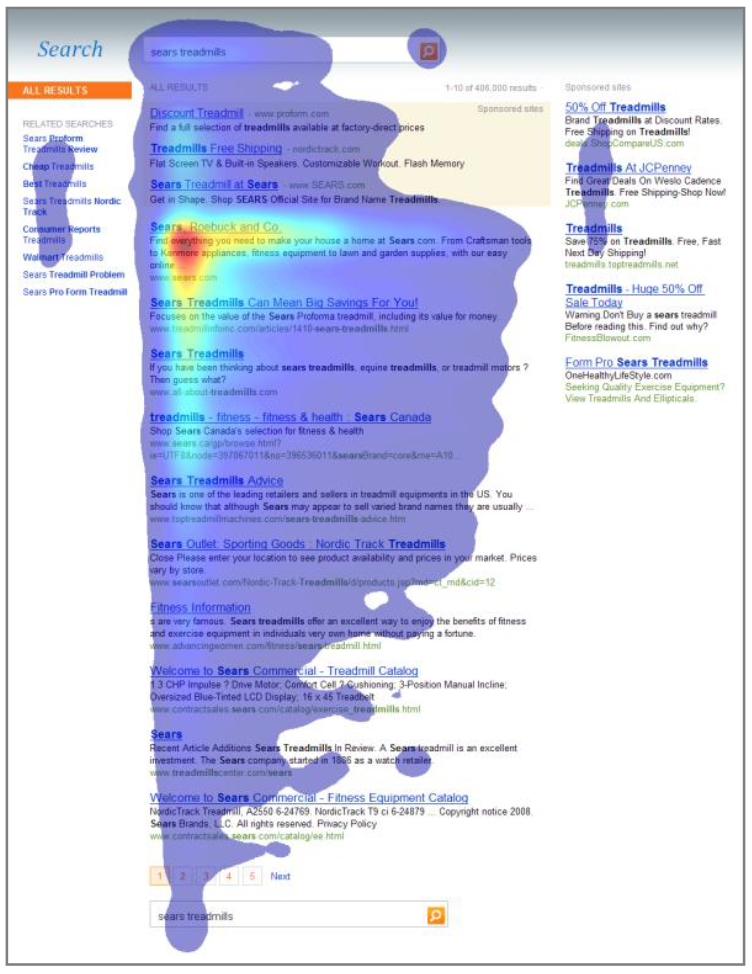
\includegraphics[width=1 \linewidth]{images/SERP_buscher2010good.png}
    \caption{
        Modern SERP that is overlapped with a heat map to represent the fixations executed by users \autocite[42]{buscher2010good}
    }
    %for reference to this figure
    \label{figure:Serp}
\end{figure}



\section{Discussion}
\label{section:Discussion}
Discussion

\section{Conclusion}
\label{section:Conclusion}
Since recording the user's eyes with an eye tracking device has been a helpful advantage for improving search engines, the primary focus lays on eye tracking \autocite{liu2015influence}. Therfore, in this paper, the most common eye tracking technologies, parameters and also visualization methods were presented. Furthermore, this paper discusses important conventions concerning modern commercial search engines. The goal was to get a better understanding of how the user looks at a search engine result page and processes the presented results \autocite{biedert2010eyebook}.

As mentioned before, modern SERP's consist of several sections or verticals. Nowadays, these verticals can contain various potential distractions, such as pictures, video thumbnails or simply just advertisements.   
Consequently, the user most of the times only looks at the result links and the associated abstracts. To be more accurate, the user hardly seems to look further than the first few links. Just in a few cases a person scrolls down, looks at the less relevant results, according to current algorithms, and maybe even looks at the second suggested page.
Besides the organic results, most of the users tend to look at pictures for an increased amount of time to process the displayed information.
To execute more efficient queries, a search engine should only display the organic results to avoid distractions and leave more space to explore more of the many suggested results.

Most of the research that has been done is based on the same theories or hypotheses, and therefore also the same parameters and visualization methods. 
Although a lot of research already exists, future research should include a broader range of parameters as a standard to examine search engines. Furthermore, it should include direct comparisons between popular commercial and non-commercial search engines.



